\chapter{Конструкторская часть}
В этом разделе будут представлены схемы алгоритмов конвейрной и линейной обработки текста.


\section{Разработка алгоритмов}
На рисунке \ref{fig:linear} представлена схема алгоритма линейной обработки текста. 
На рисунках \ref{fig:parallel} схема алгоритма конвейерной обработки текста, а на рисунках \ref{fig:thread1}-\ref{fig:thread3} --- схемы потоков обработки текста (ленты конвейера).

\begin{figure}[h!]
	\centering
	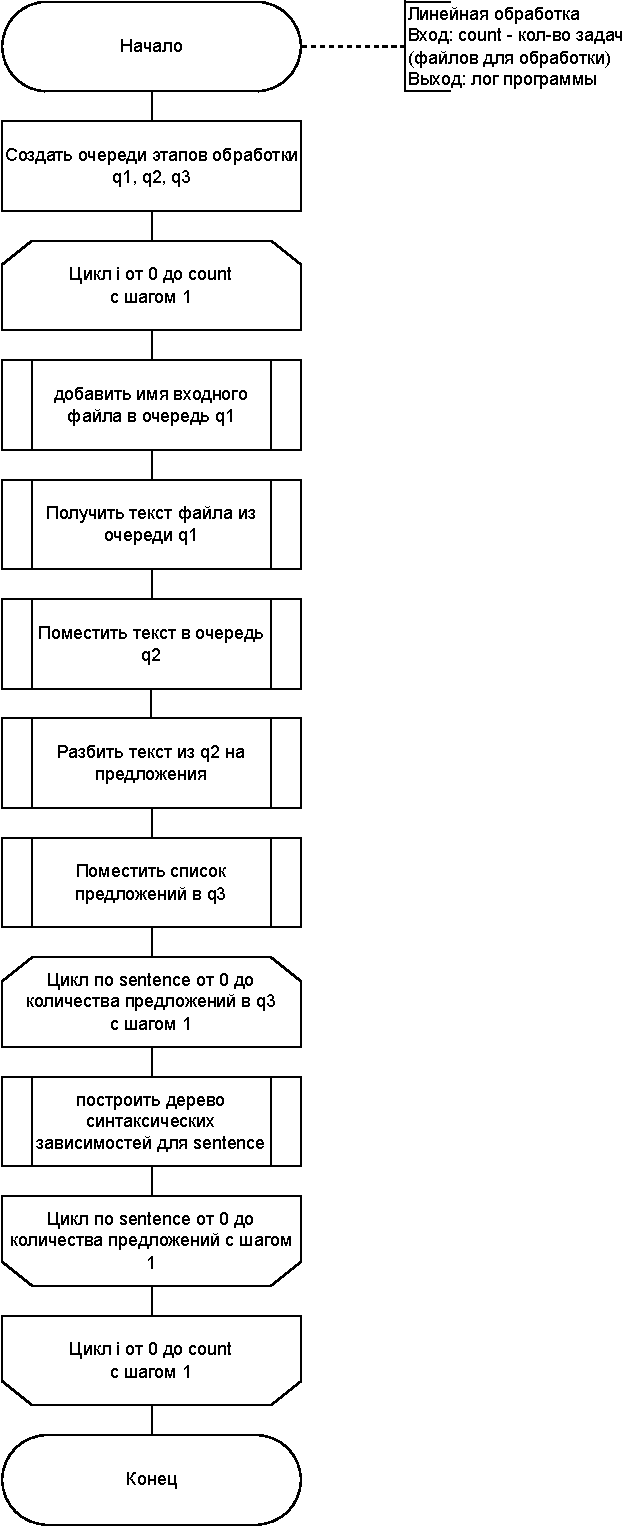
\includegraphics[width=0.6\linewidth]{img/linear}
	\caption{Схема алгоритма линейной обработки матрицы}
	\label{fig:linear}
\end{figure}

\begin{figure}[h!]
	\centering
	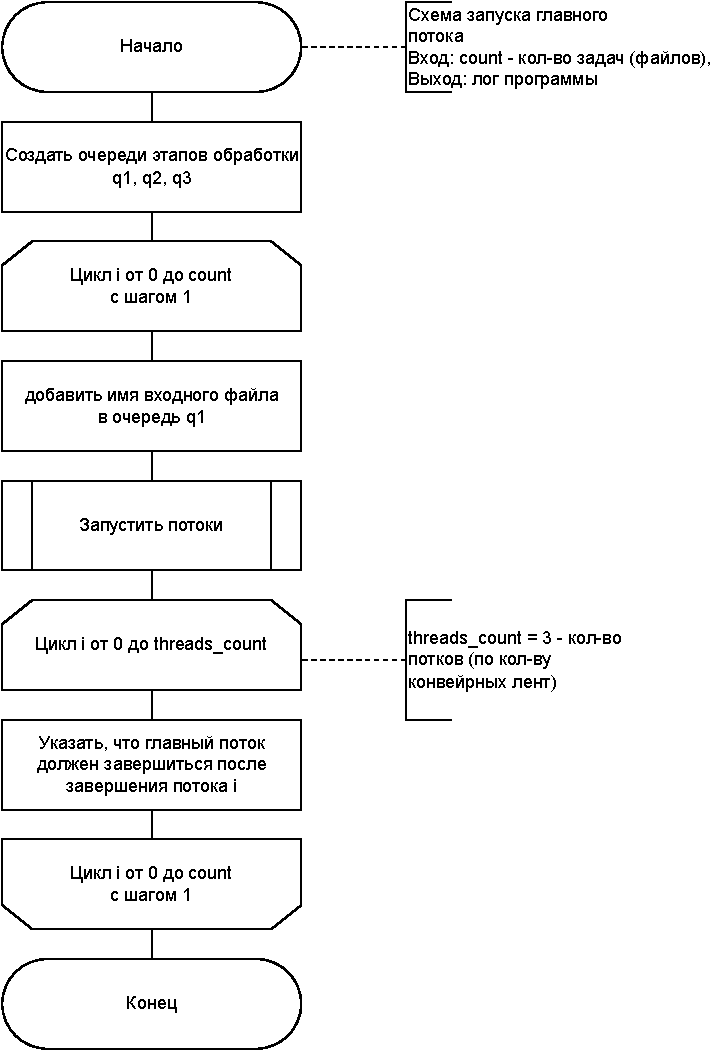
\includegraphics[width=0.78\linewidth]{img/parallel}
	\caption{Схема конвейерной обработки матрицы}
	\label{fig:parallel}
\end{figure}

\begin{figure}[h!]
	\centering
	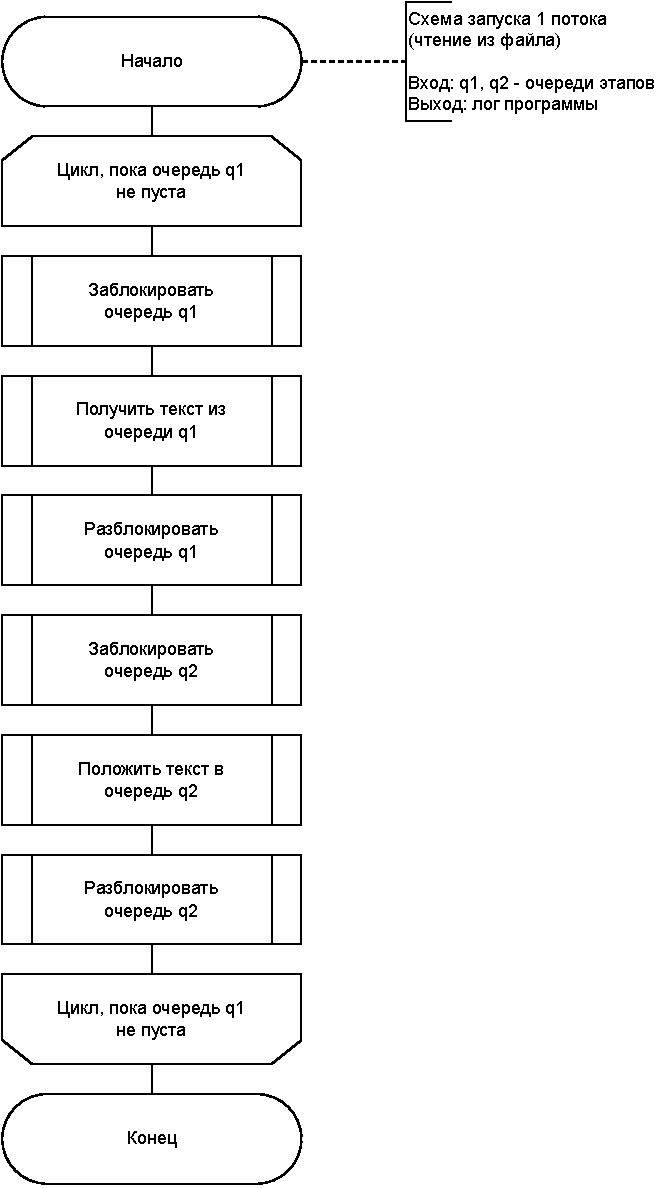
\includegraphics[width=0.78\linewidth]{img/thread1}
	\caption{Схема 1 потока обработки матрицы --- чтение текста из файла}
	\label{fig:thread1}
\end{figure}

\begin{figure}[h!]
	\centering
	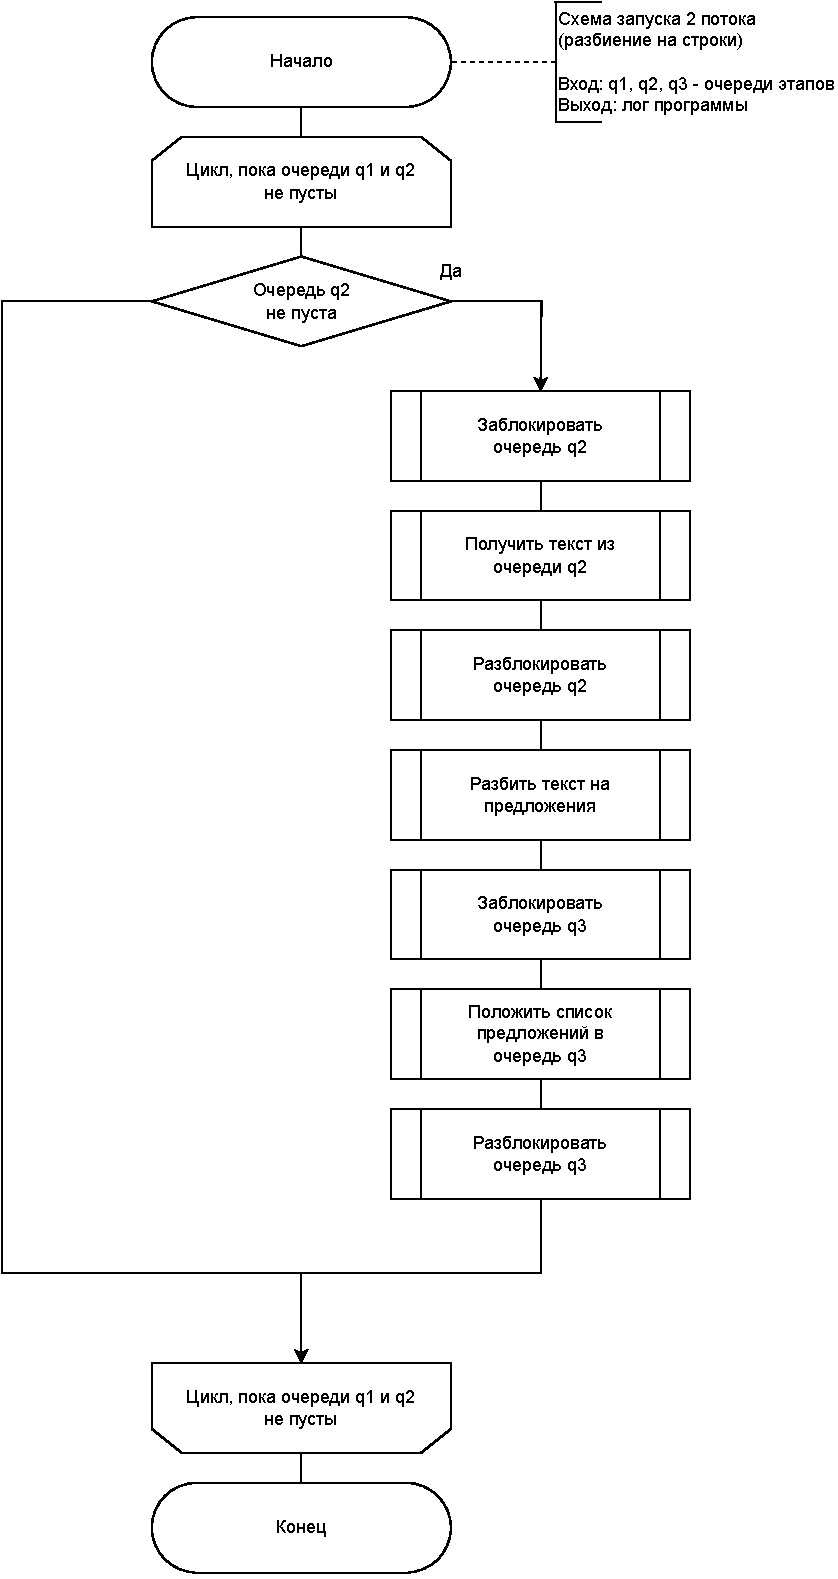
\includegraphics[width=0.75\linewidth]{img/thread2}
	\caption{Схема 2 потока обработки матрицы --- разбиение текста на предложения}
	\label{fig:thread2}
\end{figure}
\clearpage
\begin{figure}[h!]
	\centering
	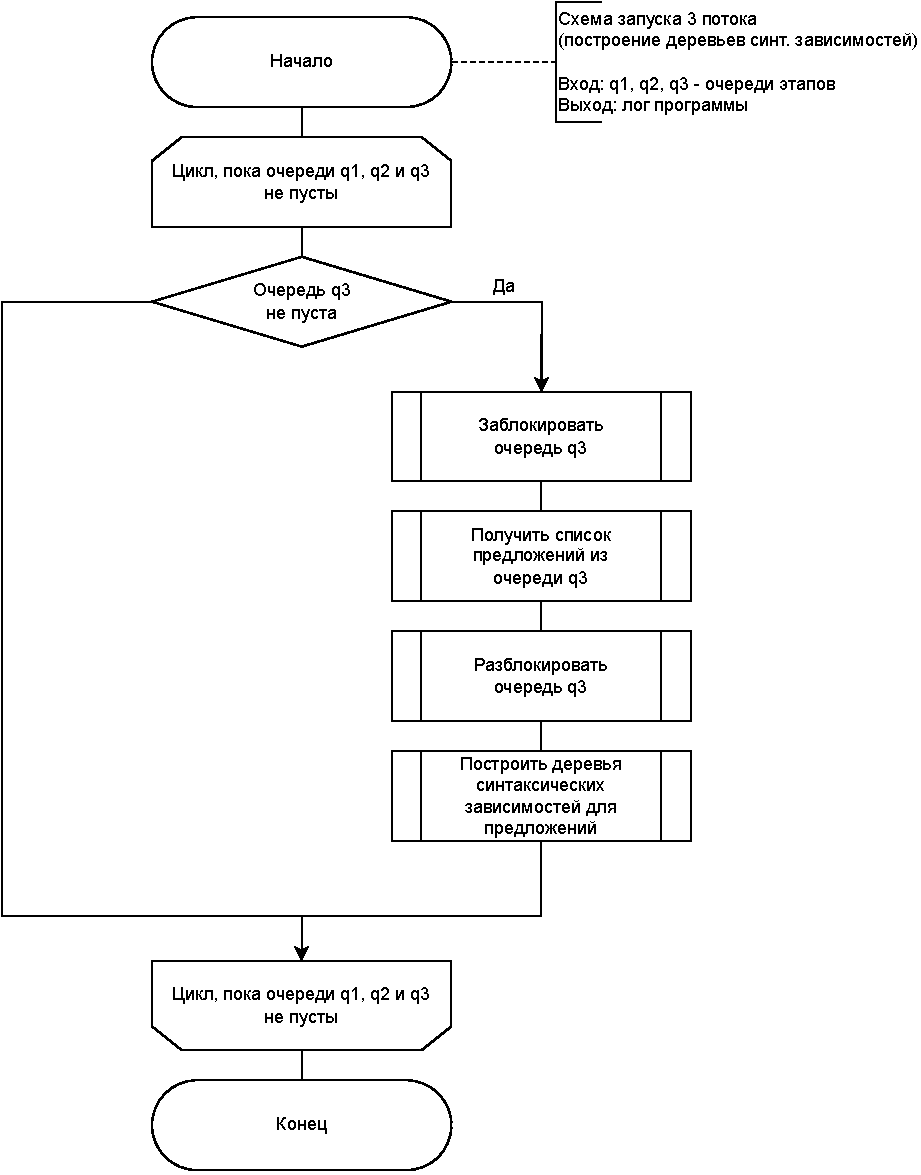
\includegraphics[width=0.78\linewidth]{img/thread3}
	\caption{Схема 3 потока обработки матрицы --- построение деревьев синтаксических зависимостей}
	\label{fig:thread3}
\end{figure}



\section{Вывод}

В данном разделе были построены схемы алгоритмов, рассматриваемых в лабораторной работе.
